%----------------------------------------------------------------------------
\chapter{Rendszer felépítése}
\label{sec:system}
%----------------------------------------------------------------------------
Ebben a fejezetben szeretném bemutatni az általam elkészített rendszert és az azt alkotó egyes részeket.


%----------------------------------------------------------------------------
\section{Rendszer részei}
%----------------------------------------------------------------------------
Az elkészült rendszer három fő komponensből áll. Ezek együttesen képesek tetszőleges tulajdonsággal rendelkező szolgáltatás hálózatokat megvalósítani, azt Kubernetes alatt elindítani, forgalmat generálni és mérés során adatokat gyűjteni. 

Az egyes részekről bővebben is lesz szó, azonban most átfogóan ismertetem a rendszert, ami a \ref{fig:system_overview} ábrán látható. Minden elem megalkotásánál egy lényeges szempont volt, hogy az elkészült rendszerrel könnyen lehessen méréseket indítani és a lehető legtöbb paraméter konfigurálható legyen.

A mérések paramétereit egy konfigurációs fájlban tudjuk megadni, ahonnan egy python program olvassa be és vezényli le a mérések elvégzését. Előszőr a Kubernetes API-n keresztül létrehoz egy \textit{ServiceGraph} objektumot. Ez nem egy beépített típus, úgyhogy a Kubernetes nem tud vele mit kezdeni ezért írni kellett egy operátort, ami képes egy ilyen definíció szerint létrehozni a szükséges erőforrásokat (\textit{deployment, pod, service, HPA}). Ahhoz, hogy az egyes kiszolgáló egységeket is tudjuk tetszés szerint konfigurálni kell egy olyan képfájl, ami a megadott paraméterek alapján tud működni. Ezért írni kellett egy külön alkalmazást hozzá.

Miután elkészültek a kért objektumok és képesek már kiszolgálni a klaszteren kívülről érkező igényeket a python szkript elkezd forgalmat generálni. A terhelés lejárta után ki kell nyerni a mérés során keletkezett adatokat. Ebben egy külön szoftver segít a Prometheus\citep{Prometheus}. 

Az elkészült rendszerhez szükséges részek forráskódjai megtalálhatóak a GitHub felületén\citep{gitRepo}. 

% Rendszer áttekintése -------------------------------------------------------
\begin{figure}[!ht]
\centering
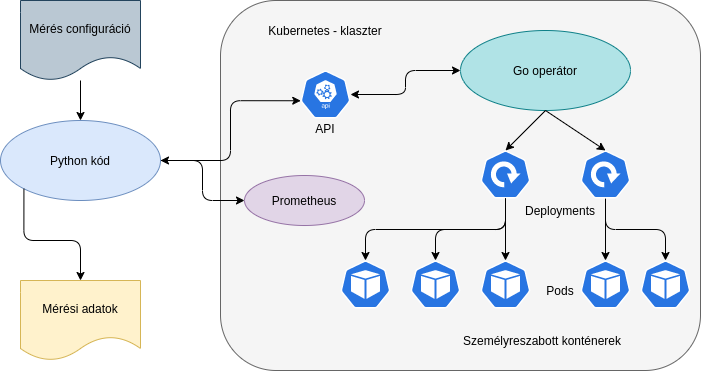
\includegraphics[width=150mm, keepaspectratio]{figures/system_overview.png}
\caption{Rendszer áttekintése}
\label{fig:system_overview}
\end{figure}

%----------------------------------------------------------------------------
\section{Korábbi munkák}
%----------------------------------------------------------------------------
A korábbi proejekttárgyak keretén belül már foglalkoztam hasonló kérdéskörrel, így már volt az egyes eszközök használatához tapasztalat és implementáció is, amiből tovább lehetett haladni. 
Önálló labor tárgyban megismerkedtem a Go programozási nyelvvel, és elkészítettem egy Kubernetes operátort, ami képes egyedi erőforrás definíciók feldolgozására és ezalapján képes beépített objektumokat létrehozni.

Korábban készítettem már egy Docker képfájl is, ami a jelenlegi rendszerben felhasználttal azonos céllal születet, hogy szabadon konfigurálható paraméterezés alapján szolgálja ki a beérkező kéréseket.

%----------------------------------------------------------------------------
\section{Operátor}
%----------------------------------------------------------------------------
Fontos szempontnak tekintettük, hogy egyszerű konfigurációs fájl alapján létre lehessen hozni a szolgáltatáhálót, amit szeretnénk tesztelni. 
Mivel a Kubernetes fejlesztők tudták, hogy nem tudnak minden igényt kiszolgálni gondoltak arra, hogy a rendszer könnyen kibővíthető legyen. Az operátorok pont erre valóak. Létrehozásukkal külön logikát tudunk implementálni, ami egy egyedi Kubernetes erőforrás objektumra figyel. 

%TODO

\subsection{Működése}
%----------------------------------------------------------------------------
A \ref{servicegraph_example} kódrészlet mutat egy példát a szolgáltatásháló definíciójára. Számunkra elég végiggondolni, hogy milyen szolgáltatásokat szeretnénk, hogyan kövessék egymást, milyen erőforrást biztosítsunk számukra. Miután ezek megvannak készítünk belőle egy \textit{yaml} dokumentumot.

Látható, hogy a \verb+apiVersion+ és \verb+kind+ érték egyedi, így tudunk hivatkozni a saját erőforrásunkra. Szintén meg kell adni pár meta információt, mint például az objektum neve és névtere. A \verb+spec+ szekció az érdekes számunkra. Itt tudjuk felsorolni, hogy milyen szolgáltaásokat szeretnénk majd a hálózatba. Be tudjuk állítani, hogy hány replikával fusson egy-egy szolgáltatás, illetve hogy milyen portokon tudjuk majd őket elérni. Ezek az információk azért lesznek fontosak, mert ezalapján fog az operátor létrehozni Kubernetes Deploymenteket és Serviceket. Ha szeretnénk skálázást is beállítani az adott szolgáltasra akkor azt is megtehetjük, ha megadjuk a \verb+hpa+ konfigurációs paramétereket. Ezek hiányában nem kerül létrehozásra, és fix replikaszámmal fog üzemelni.

Továbbá definiálni kell, hogy az adott szolgáltatás milyen végpontok hívására figyeljen. Például a \textit{front-end} szolgáltatás a \verb+/instant+ és \verb+/chain+ lekérdezésekre fog válaszolni. A válasz gyorsasága és a közben felhasznált erőforrás mennyiséget is lehetőségünk van befolyásolni. Az itt magadott paraméterek továbbításra kerülnek majd a futtatot konténerekhez így ők fogják helyileg érvényre juttatni a szabályokat. 

A bemutatott kód csak részlete a teljes forrásállománynak, mert elég repetitiv ezért nem szerettem volna a helyet foglalni, de a GitHub repóban megtalálható a teljes kód. \\

\lstset{caption=Saját szolgáltatásháló definiálása, label=servicegraph_example}
\lstinputlisting{figures/servicegraph.yaml}

Miután megtörtént a szolgáltatásháló leírása és fut a korábban elkésztett operátor könnyű dolgunk van. Mintha csak egy beépített erőforrást hoznánk létre a \ref{servicegraph_apply} kódrészletben mutatott módon telepíthető is. 
Ilyenkor az történik, hogy a \verb+kubectl+ parancs a Kubernetes API-ját meghívja, és továbbítodik az operátor felé. Az operátor kiolvassa a kapott objektum értékeit és ezalapján létrehozza a kívánt erőforrásakat. 

\lstset{caption=Szolgáltatásháló indítása, label=servicegraph_apply}
\begin{lstlisting}[language=bash,morekeywords={kubectl, apply},alsoletter={-},breaklines=true]
$ kubectl apply -f path/to/servicegraph.yaml                          
servicegraph.dipterv.my.domain/servicegraph created 
\end{lstlisting}


Operetaor sdk, tavalyiról már megvolt a váza, Hibákkal működött, HPA bele rakni, kisebb változatatások. Létrehoz Deploymenteket --> podok, Servicek, 
A konténereket is azalapján indítja, paraméterezi.go nyelven
Hogyan működik: API, CRD, CR.

%----------------------------------------------------------------------------
\section{Go konténer}
%----------------------------------------------------------------------------
A korábban látott módon lehetőségünk van tetszőleges szolgáltaásokat elindítani, azonban hogy az adott szolgáltatásoknak további paraméterek tudjunk átadni, olyan alkalmazás kell ami tudja kezelni őket. Például: milyen végpontokra figyeljenek, milyen kiszolgálási idővel dolgozzanak, mennyi erőforrást használjanak fel. Erre a feladatra létrehoztam külön egy Go alapú webalkalmazást. 
A paraméterek átadására indításkor van lehetőség és futás közben figyelembe veszi ezeket. Beépítettként tartalmaz egy processzor intenzív algoritmust, amit magadott alkalommal lefuttat egy-egy kérés során. 

%TODO

%----------------------------------------------------------------------------
\section{Mérés vezénylése}
\label{sec:measure_orchestrate}
%----------------------------------------------------------------------------
Az elkészített operátorral és konténerizált alkalmazásunkkal tetszőleges szolgáltatáshálót képesek vagyunk létrehozni.
Azonban a mérések elvégzése így is nehéz feladat, mert szeretnénk, hogy determinisztikus legyen. Itt is fontos szempont volt, hogy a lehető legegyszerűbben és a rugalmasa módon lehessen végezni a méréseket. 
A feladat megvalósításához a Python nyelvet választottam, mivel könnyen lehet benne fejleszteni és komoly számítást nem végez így nem számottevő a plusz erőforrásfelhasználása más, alacsonyabb szintű nyelvekhez képest. 

Mérés megkezdése előtt készíteni kell egy konfigurációs fájlt. Erre egy példa látható a \ref{measurement_config} kódrészleten. A mérést vezénylő alkalmazás az itt megadott paraméterek alapján fogja végezni a mérést. Többek között meg kell adni, hogy a mérések milyen szolgáltatáshálózatokon kerüljenek elvégzésre. Lehetőség van többet is megadni, így egy indítással akár az összes számunkra érdekes esetet le tudjuk szimulálni egyszerre. Továbbá meg kell adni, hogy milyen kérés per másodperc (\textit{QPS}) értékekre vagyunk kíváncsiak. Fontos megadni, hogy milyen forgalmat és hova szeretnénk generálni. Ez látható a \verb+Load+ részen belül. Megadjuk a mérés idejét, IP címet és portot, ahol a szolgáltatásunk fogja fogadni a kéréseket.\\


\lstset{caption=Mérés konfigurációja, label=measurement_config}
\lstinputlisting{figures/measurement_config.yaml}

A forgalom generálását egy külön alkalmazás végzi, a \verb+Fortio+. Egyre szélesebb körben elterjedt forgalom generáló alkalmazást azért válaszztottuk, mert elég sok statisztikát képes gyűjteni és könnyen kezelhető, ezáltal könnyen integrálható a rendszerünkbe. Egy valódi indítást mutat be a  \ref{fortio_command} kódrészlet. 
Látható, hogy meg kell adni az aktuális QPS értéket, amit szeretnénk elérni, hogy mennyi idig fusson a mérés, hogy hova és milyen néven mentse a kapott eredményeket, és a legfontosabb, hogy hova küldje a kéréseket.
Ezeket a paramétereket ugye a korábban ismertetett konfigurációs fájl alapján állítjuk össze. \\

\lstset{caption=Példa a \textit{Fortio} indítására, label=fortio_command}
\lstinputlisting[language=Bash]{figures/fortio_command.sh}

Miután megterheltük a rendszert és megkaptuk a kérések kiszolgálásával kapcsolatos statisztikákat a \verb+Fortio+-ból, szükséges még a rendszer erőforrásfelhasználását célzó metrikálkat is begyűjteni. 
Erre a \verb+Prometheus+ rendszerén keresztül van lehetőségünk.
A szoftver támogatja az API hívásokat, így lehetőségünk nyílik könnyen lekérdezni az általa gyűjtött statisztikákat. 

A metrikák lekérdezésére a \ref{prometheus_query} kódrészlet ad egy példát. Meg kell adnunk, hogy milyen értékekre vagyunk kíváncsiak. A látható példában ez a konténerek által felhasznált CPU mennyisége, továbá kitöséket teszünk, hogy csak a \textit{Default} vagy \textit{Metrics} névtérben futó konténerek érdekelnek.
Meg kell adni a lekérdezés kezdeti és vég idejét, ez ugye az lesz amíg a generált kéréseket kiszolgálta.
Össze kell állítani a \verb+Prometheus+ elérhetőségét, amihez a mérés elején megadott konfigurációt vesszük alapul. Ha megvan az előkészített API hívás, akkor a kódrészletben látott módon meg kell hívni azt. A kapott választ \verb+json+ formátumban érkezik, így később mi is így kezeljük. \\


\lstset{caption=\textit{Prometheus} rendszer használata python kódból, label=prometheus_query}
\lstinputlisting{figures/prometheus.py}

A korábban látott megoldással egyéb adatokat is metrikákat is lekérdezhetünk. Jelenleg négy értéket gyűjtünk:
\begin{itemize}
  \item Konténerek processzor felhasználásait külön-külön.
  \item Konténerek memória felhasználásait külön-külön.
  \item Az összes futó \textit{Pod}, ami részt vesz a mérésben.
  \item A futó konténerek száma típus szerint. (például: külön amik a frontend szolgáltatást valósítják meg és külön amik a backend szolgáltatást)
\end{itemize}

A \verb+Prometheus+ egészen kiterjeszthető rendszer így közel tertszőleges metrikákat lehet gyűjteni. 


A mérés végén miután összegyűjtöttük az összes keletkező adatokat, beleértve a \verb+Prometheus+ és \verb+Fortio+ rendszereket is és az eredeti konfigurációt is azokat perzisztálni kell. Erre a legkézenfekvőbb módszer az adatok kiírása \verb+json+ fájlba. Ez azért is előnyös, mert könnyen olvasható és feldolgozható a formátum. 